\providecommand{\tituloDocumento}{Guía}
\providecommand{\subtituloDocumento}{Elementos secundarios del triángulo}

\documentclass{sn-guia}

\begin{document}
%
\raggedright
\begin{tcbraster}[enhanced,raster columns=2,raster width=\linewidth,raster column skip=3pt,raster force size=false]
    \begin{caja}[title={\sffamily\scshape\bfseries Nombre},height=30pt,add to width=4cm]
    \end{caja}
    \begin{caja}[title={\sffamily\scshape\bfseries Curso},height=30pt,add to width=-4cm]
    \end{caja}    
    \begin{caja}[title={\sffamily\scshape\bfseries Fecha},height=30pt]
    \end{caja}                
    \begin{caja}[title={\sffamily\scshape\bfseries Profesor},height=30pt]
    \end{caja}
\end{tcbraster}
\vspace*{5mm}


\section*{Transversal de gravedad}
Es la recta que une un vértice con el punto medio del lado opuesto. Se denominan $t_a$, $t_b$ y $t_c$; donde el 
subíndice indica el vértice por el cual pasa. Las tres transversales de gravedad se interceptan en un mismo punto 
llamado Centro de Gravedad (o Baricentro).

\begin{tcolorbox}[blanker,sidebyside]
    \begin{center}
        \begin{tikzpicture}[ampersand replacement=\&, line width=1pt]
            \draw (0,0) coordinate[label=below:$A$] (A) -- (7,0) coordinate[label=below:$B$] (B) %
            -- ([turn]150:6) coordinate[label=above:$C$] (C) -- cycle; 
            \draw[name path=ta] (A) -- ($(B)!0.5!(C)$) node [above,pos=0.3] {$t_a$} node [right,yshift=3pt,pos=1] {$D$};
            \draw[name path=tb] (B) -- ($(C)!0.5!(A)$) node [above,pos=0.3] {$t_b$} node [left,pos=1] {$E$}; 
            \draw (C) -- ($(A)!0.5!(B)$) node [right,pos=0.3] {$t_c$} node [below,pos=1] {$F$};
            \draw[name intersections={of=ta and tb, by=G},fill] (G) circle (1pt) node [below=3pt,xshift=-3pt] {$G$};
        \end{tikzpicture}
    \end{center}
    \tcblower
    \begin{itemize}
        \item D, E, F: Puntos medios de los lados.
        \item $\overline{AD} = t_a$; $\overline{BE} = t_b$; $\overline{CF} = t_c$.
        \item $t_a \cap t_b \cap t_c = \left\{G\right\}$.
        \item $G$: Centro de Gravedad (o Baricentro).
    \end{itemize}
\end{tcolorbox}

\subsection*{Propiedad} 
El Baricentro divide cada transversal de gravedad en dos segmentos que están en la razón 2:1. El segmento que
va desde el vértice al Baricentro mide el doble que el segmento va desde el Baricentro al lado.

\section*{Altura}
Es la perpendicular bajada desde un vértice al lado opuesto. Se denomina $h_a$, $h_b$, y $h_c$; donde el
subíndice indica el vértice por el cual pasa. Las tres alturas se interceptan en un mismo punto llamado
Ortocentro.  

\begin{tcolorbox}[blanker,sidebyside]
    \begin{center}
        \begin{tikzpicture}[ampersand replacement=\&, line width=1pt]
            \draw (0,0) coordinate[label=below:$A$] (A) -- (6,0) coordinate[label=below:$B$] (B) %
            -- ([turn]120:6) coordinate[label=above:$C$] (C) -- cycle; 
            \draw[name path=ha] (A) -- ($(B)!0.5!(C)$) node [above left,pos=0.4] {$h_a$} node [right,yshift=3pt,pos=1] {$D$};
            \draw[name path=hb] (B) -- ($(C)!0.5!(A)$) node [above right,pos=0.4] {$h_b$} node [left,pos=1] {$E$}; 
            \draw (C) -- ($(A)!0.5!(B)$) node [right,pos=0.4] {$h_c$} node [below,pos=1] {$F$};
            \draw[name intersections={of=ha and hb, by=H},fill] (H) circle (1pt) node [below right=3pt,xshift=-4pt,yshift=-2pt] {$H$};
        \end{tikzpicture}
        \end{center}
    \tcblower
    \begin{itemize}
        \item $\overline{AD} \perp \overline{BC}$ ; $\overline{BE} \perp \overline{CA}$ ; $\overline{CF} \perp \overline{AB}$.
        \item $\overline{AD} = h_a$; $\overline{BE} = h_b$; $\overline{CF} = h_c$.
        \item $h_a \cap h_b \cap h_c = \left\{H\right\}$.
        \item $H$: Ortocentro.
    \end{itemize}
\end{tcolorbox}

\subsection*{Propiedad} 
Las alturas de un triángulo son inversamente proporcionales a los lados. Es decir,
\begin{equation*}
    a\cdot h_a = b\cdot h_b = c \cdot h_c = k\;.
\end{equation*}

\subsection*{Observaciones}
{\textbullet} En un triángulo obtusángulo, el ortocentro queda en el exterior del triángulo.
\begin{center}
\begin{tikzpicture}[ampersand replacement=\&,line width=1pt]
    \draw (0,0) coordinate[label={[label distance=5mm]100:$A$}] (A) -- (30:4) coordinate[label=above:$B$] (B) -- ([turn]140:8) coordinate[label=above:$C$] (C) -- cycle;
    \path[name path=hc] (C) -- ($(A)!(C)!(B)$) -- ([turn]0:4cm);
    \path[name path=hb] (B) -- ($(A)!(B)!(C)$) -- ([turn]0:4cm);
    \draw[name intersections={of=hc and hb,by=H}] (H) circle (1pt) node [below] {$H$};
    \draw ($(B)!(A)!(C)$) -- (H) node [pos=0.2,right] {$h_a$};
    \draw (B) -- (H) node [midway,right] {$h_b$};
    \draw (C) -- (H) node [midway,left] {$h_c$};
    \draw (B) -- ($(C)!(B)!(H)$) -- ([turn]90:5pt) -- ([turn]90:5pt) -- ([turn]90:5pt);
    \draw (C) -- ($(H)!(C)!(B)$) -- ([turn]90:5pt) -- ([turn]90:5pt) -- ([turn]90:5pt);
    \draw (A) -- ($(C)!(A)!(B)$) -- ([turn]90:5pt) -- ([turn]90:5pt) -- ([turn]90:5pt);
\end{tikzpicture}
\end{center}

{\textbullet} En un triángulo rectángulo, el ortocentro coincide con el vértice del ángulo recto, puesto
que los catetos se confunden con las alturas.

\begin{center}
\begin{tikzpicture}[ampersand replacement=\&,line width=1pt]
    \draw (0,0) coordinate [label=below:C] (C) -- (6,0) coordinate [label=right:A] (A) -- (0,4) coordinate [label=above:B] (B) -- cycle;
    \node [left] at ($(B)!0.5!(C)$) {$h_b$};
    \node [below] at ($(A)!0.5!(C)$) {$h_a$};
    \draw (C) -- ($(A)!(C)!(B)$) node [midway,below right] {$h_c$} -- ([turn]90:5pt) -- ([turn]90:5pt) -- ([turn]90:5pt);
    \draw (C) -- ([turn]90:5pt) -- ([turn]90:5pt) -- ([turn]90:5pt);
\end{tikzpicture}
\end{center}

\section*{Bisectriz}

Es la recta que pasa por el vértice y divide al ángulo en dos partes iguales. Se denominan $b_a$, $b_b$ y $b_c$; donde el 
subíndice indica el ángulo que divide. Las tres Bisectrices se interceptan en un mismo punto llamado Incentro, el cual 
corresponde al centro de la circunferencia inscrita al triángulo, es decir, el incentro equidista de los lados del triángulo. 

\begin{tcolorbox}[blanker,sidebyside] 
    \begin{center}
    \begin{tikzpicture}[ampersand replacement=\&,line width=1pt]
        \draw (0,0) coordinate [label=below:$A$] (A) -- (6,0) coordinate [label=below:$B$] (B) % 
        --  ([turn]120:5) coordinate [label=above:$C$] (C) -- cycle;
        %%% bisectriz en A
        \path[name path=ba] let \p{ab} = ($(A)!1cm!(B)$), \p{ac} = ($(A)!1cm!(C)$) in
            (A) -- ($(\p{ab})!0.5!(\p{ac})$) -- ([turn]0:5cm);
        \path[name path=BC] (B) -- (C);
        \node [name intersections={of=ba and BC, by=F},above right] at (F) {$F$};
        \draw (A) -- (F);
        %%% bisectriz en B
        \path[name path=bb] let \p{ba} = ($(B)!1cm!(A)$), \p{bc} = ($(B)!1cm!(C)$) in
        (B) -- ($(\p{ba})!0.5!(\p{bc})$) -- ([turn]0:5cm);
        \path[name path=AC] (A) -- (C);
        \node [name intersections={of=bb and AC, by=G},above left] at (G) {$G$};
        \draw (B) -- (G);
        %%% bisectriz en C
        \path[name path=bc] let \p{ca} = ($(C)!1cm!(A)$), \p{cb} = ($(C)!1cm!(B)$) in
            (C) -- ($(\p{ca})!0.5!(\p{cb})$) -- ([turn]0:5cm);
        \path[name path=AB] (A) -- (B);
        \node [name intersections={of=bc and AB, by=E},below] at (E) {$E$};
        \draw (C) -- (E);
        %% incirculo
        \node [name intersections={of=ba and bb,by=I},draw, circle through=(F)] at (I) {};
        \node [label=70:$I$] at (I) {};
        %% cuadraditos de 90 grados
        \draw (E) -- ($(E)!5pt!(B)$) -- ([turn]90:5pt) -- ([turn]90:5pt);
        \draw (F) -- ($(F)!5pt!(C)$) -- ([turn]90:5pt) -- ([turn]90:5pt);
        \draw (G) -- ($(G)!5pt!(A)$) -- ([turn]90:5pt) -- ([turn]90:5pt);
    \end{tikzpicture}
    \end{center}
\tcblower
        \begin{itemize}[]
            \item $\overline{AF} = b_a$; $\overline{BG} = b_b$; $\overline{CE} = b_c$.
            \item $b_a \cap b_b \cap b_c = \left\{I\right\}$.
            \item $I$ : Incentro.
            \item $\frac{\overline{AE}}{\overline{AC}} = \frac{\overline{BE}}{\overline{BC}}$; %
            $\frac{\overline{AG}}{\overline{AB}} = \frac{\overline{CG}}{\overline{BC}}$; %
            $\frac{\overline{BF}}{\overline{AB}} = \frac{\overline{CF}}{\overline{AC}}$; 
        \end{itemize}
\end{tcolorbox}

\subsection*{Observación}
En general, los puntos de tangencia de los lados con la circunferencia inscrita al 
triángulo no coinciden con los pies de las Bisectrices.

\section*{Simetral}
Es una recta perpendicular al lado del triángulo que pasa por su punto medio. Las simetrales se 
designan por: $S_a$, $S_b$ y $S_c$; donde el subíndice indica el lado al cual es perpendicular.

El punto de intersección se denomina Circuncentro y corresponde al centro de la circunferencia
circunscrita al triángulo, es decir, el circuncentro es un punto que equidista de los 
tres vértices del triángulo. 

\begin{tcolorbox}[blanker,sidebyside]
    \begin{center}
    \begin{tikzpicture}[ampersand replacement=\&,line width=1pt]
        \node [draw,shape=circle,inner sep=20mm,name=circulo] at (0,0) {};
        \draw (circulo.214) coordinate [label=below left:$A$] (A) -- (circulo.330) coordinate [label=below right:$B$] (B) % 
        -- (circulo.70) coordinate [label=above right:$C$] (C) -- cycle;
        \draw[] (0,0) -- (circulo.20) node [pos=0.4,below] {$S_a$};
        \draw[] (0,0) -- (circulo.142) node [pos=0.7,above right] {$S_b$};
        \draw[] (0,0) -- (circulo.272) node [pos=0.3,left] {$S_c$}; 
        \draw ($(A)!(0,0)!(B)$) node [below right] {$E$} -- ([turn]90:5pt) -- ([turn]90:5pt) -- ([turn]90:5pt);
        \draw ($(B)!(0,0)!(C)$) node [xshift=10pt,yshift=-5pt] {$D$} -- ([turn]90:5pt) -- ([turn]90:5pt) -- ([turn]90:5pt);
        \draw ($(C)!(0,0)!(A)$) node [xshift=-10pt,yshift=-2pt] {$F$} -- ([turn]90:5pt) -- ([turn]90:5pt) -- ([turn]90:5pt);
        \node [below right] at (0,0) {$O$};
    \end{tikzpicture}
    \end{center}
    \tcblower
     \begin{itemize}
        \item $\overline{OD}=S_a$; $\overline{OF}=S_b$; $\overline{OE}=S_c$.
        \item $S_a \cap S_b \cap S_c = \left\{O\right\}$.
        \item $O$: Circuncentro.
     \end{itemize}
\end{tcolorbox}

\subsection*{Observación}

En general, las simetrales no pasan por los vértices del triángulo.

\section*{Mediana} 
Es el segmento de recta que une los puntos medios de dos lados del triángulo.

\begin{tcolorbox}[blanker,sidebyside]
    \begin{center}
    \begin{tikzpicture}[ampersand replacement=\&,line width=1pt]
        \draw (0,0) coordinate [label=below:$A$] (A) -- (6,0) coordinate [label=below:$B$] (B) % 
        -- (40:5) coordinate [label=above:$C$] (C) -- cycle;
        \draw ($(A)!0.5!(B)$) coordinate [label=below:$Q$] (Q) -- ($(B)!0.5!(C)$) coordinate [label=above right:$R$] (R) % 
        -- ($(C)!0.5!(A)$) coordinate [label=above left:$P$] (P) -- cycle;
    \end{tikzpicture}
    \end{center}
    \tcblower
        \begin{itemize}
            \item $P$, $Q$, $R$: Puntos medios de los lados.
            \item $\overline{PQ}$, $\overline{QR}$, $\overline{RP}$: Medianas 
        \end{itemize}
\end{tcolorbox}

\subsection*{Propiedades}
\begin{itemize}
    \item La mediana es paralela al tercer lado: $\overline{RP}\parallel\overline{AB}$, $\overline{QR}\parallel\overline{AC}$ y
    $\overline{PQ}\parallel\overline{BC}$.
    \item La mediana mide la mitad del lado al cual es paralela:
    $\overline{AB}=2\cdot\overline{PR}$, $\overline{BC}=2\cdot\overline{PQ}$ y $\overline{AC}=2\cdot\overline{QR}$.
    \item Cuando se dibujan las tres medianas de un triángulo, se forman cuatro
    triángulos congruentes.
\end{itemize}

\section*{Teorema de Pitágoras}
\begin{tcolorbox}[blanker,sidebyside,lefthand ratio=0.7]
  `` En todo triángulo $ABC$ rectángulo en C, se cumple que el cuadrado de la hipotenusa es igual a la suma de los
  cuadrados de los catetos, es decir, $a^2 + b^2 = c^2$ . '' 
    \tcblower
    \begin{center}
    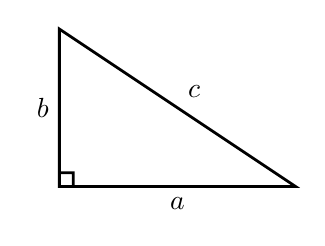
\begin{tikzpicture}[ampersand replacement=\&,line width=1pt]
        \draw (0,0) -- node [midway,below] {$a$} (3,0) -- node [midway,above right] {$c$} (0,2) -- node [midway,left] {$b$} cycle
        -- ([turn]90:5pt) -- ([turn]90:5pt) -- ([turn]90:5pt);
    \end{tikzpicture}
    \end{center}
\end{tcolorbox}

\subsection*{Recíproco del Teorema de Pitágoras}

\begin{tcolorbox}[blanker,sidebyside,lefthand ratio=0.6]
    `` Sea un triángulo $ABC$ cualquiera, con lados menores $a$ y $b$ y lado mayor $c$, 
    tales que $c^2 = a^2 + b^2$, entonces el triángulo $ABC$ es un triángulo rectángulo. ''
    \tcblower
    \begin{center}
        {\bfseries\sffamily Tríos Pitagóricos}\vspace*{5pt}
        \begin{tblr}{colspec={ccccccc},hlines,vlines,vline{2,Z} = {1}{-}{}, vline{2,Z} = {2}{-}{}, column{even}={black!15},rowsep=2pt}
            $a$   & 3 & 5  &  8 & 7 &  20 & 12 \\ 
            $b$   & 4 & 12 & 15 & 24 & 21 & 35 \\
            $c$   & 5 & 13 & 17 & 25 & 29 & 37 \\
        \end{tblr}
        \end{center}
\end{tcolorbox}

\section*{Ejercicios}

\begin{enumerate}
    \item En el triangulo ABC rectangulo en C, $\overline{BC}=5$ [cm] y $\overline{BD}=4$ [cm]. La medida 
    de la altura $h_c$ es:

    \begin{alternativas*}[]
        \item $\dfrac{3}{2}$ [cm] 
        \item $\dfrac{9}{4}$ [cm] 
        \item $\dfrac{3}{4}$ [cm] 
        \item $4$ [cm] 
        \item $9$ [cm] 
    \end{alternativas*}

    \item En la figura, si $ABC$ y $BDF$ son triángulos equiláteros y $BFEC$ es un rombo, entonces 
    ¿Cuál(es) de las expresiones siguientes es(son) verdadera(s)?
    
    \begin{tcolorbox}[blanker,sidebyside,width=0.6\textwidth,center]
        \begin{enumerate}[label={(\Roman*)}]
            \item $x=z$
            \item $x+y= \angle EBD$
            \item $x+y-z=60^{\circ}$
        \end{enumerate}
        \tcblower
        \begin{center}
        \begin{tikzpicture}[ampersand replacement=\&,line width=1pt]
            \node [draw,regular polygon,regular polygon sides=3,minimum size=5cm,name=t] {};
            \draw (t.side 1) -- (t.side 2) -- (t.side 3) -- cycle;
            \coordinate [label=below:$A$] (A) at (t.corner 2);
            \coordinate [label=below:$D$] (D) at (t.corner 3);
            \coordinate [label=above:$E$] (E) at (t.corner 1);
            \coordinate [label=left:$C$] (C) at (t.side 1);
            \coordinate [label=below:$B$] (B) at (t.side 2);
            \coordinate [label=right:$F$] (F) at (t.side 3);
            \draw (E) -- (B);
            \draw pic ["$x$",draw,angle radius=20pt] {angle=C--B--A};
            \draw pic ["$z$",draw,angle radius=20pt] {angle=C--F--B};
            \draw pic ["$y$",draw,angle radius=35pt,angle eccentricity=0.8] {angle=B--E--D};
        \end{tikzpicture}
        \end{center}
    \end{tcolorbox}
    \begin{alternativas*}[nosep]
        \item Solo I
        \item Solo II
        \item Solo III
        \item Solo I y II
        \item I, II y III
    \end{alternativas*}
    \item Si en un triángulo equilátero se dibuja una de sus alturas, entonces se forman dos triángulos
    \begin{alternativas}[nosep]
        \item Isósceles rectángulos congruentes. 
        \item Acutángulos escalenos congruentes. 
        \item Acutángulos congruentes.
        \item Escalenos rectángulos congruentes. 
        \item Equiláteros congruentes.
    \end{alternativas}
    \item Si sobre el tercio central de uno de los lados del triángulo equilátero $ABC$ se construye otro triángulo equilátero, como se
    muestra en la figura, ¿Cuál(es) de las siguientes afirmaciones es (son) verdadera(s)?
    \begin{tcolorbox}[blanker,sidebyside,width=0.9\textwidth,center,lefthand ratio=0.65]
        \begin{enumerate}[label={(\Roman*)}]
            \item El área del $\triangle DEF$ es la sexta parte del área del $\triangle ABC$.
            \item El lado $\overline{FE}$ es paralelo al lado $\overline{AB}$.
            \item El lado $\overline{FE}$ es perpendicular al lado $\overline{AC}$.
        \end{enumerate}
        \tcblower
        \begin{center}
        \begin{tikzpicture}[ampersand replacement=\&,line width=1pt]
            \node [draw,regular polygon,regular polygon sides=3,minimum size=5cm,name=t] {};
            \coordinate[label=below:$A$] (A) at (t.corner 2);
            \coordinate[label=below:$B$] (B) at (t.corner 3); 
            \coordinate[label=above:$C$] (C) at (t.corner 1); 
            \coordinate[label=below left:$D$] (D) at ($(B)!0.33!(C)$); 
            \coordinate[label=below left:$F$] (F) at ($(B)!0.66!(C)$);
            \coordinate[label=right:$E$] (E) at ($(D)!1!-60:(F)$);
            \draw (D) -- (E) -- (F);
        \end{tikzpicture}
        \end{center}
    \end{tcolorbox}
    \begin{alternativas*}[nosep]
        \item Solo I
        \item Solo II
        \item Solo I y II
        \item Solo I y III
        \item Solo II y III
    \end{alternativas*}
    \item En la figura, $ABC$ es un triángulo equilátero de 18 cm de perímetro y $DBEC$ es un rectángulo. El área de la región sombreada es:
    \begin{tcolorbox}[blanker,sidebyside,lefthand ratio=0.2]
        \begin{alternativas}[nosep]
            \item 9 [$\textrm{cm}^{2}$]
            \item $9\sqrt{3}$ [$\textrm{cm}^{2}$]
            \item $9\sqrt{5}$ [$\textrm{cm}^{2}$]
            \item $\frac{9}{2}\sqrt{5}$ [$\textrm{cm}^{2}$]
            \item $\frac{9}{2}\sqrt{3}$ [$\textrm{cm}^{2}$]
        \end{alternativas}
        \tcblower
        \begin{center}
        \begin{tikzpicture}[ampersand replacement=\&,line width=1pt]
            \node [draw,regular polygon,regular polygon sides=3,minimum size=3cm,name=t] {};
            \coordinate[label=below:$A$] (A) at (t.corner 2);
            \coordinate[label=below:$B$] (B) at (t.corner 3);
            \coordinate[label=above:$C$] (C) at (t.corner 1);
            \coordinate[label=above right:$E$] (E) at (C -| B); %% vertical
            \draw[fill=black!30] (C) -- (E) -- (B) -- cycle;
            \coordinate[label=below:$D$] (D) at (C |- B); %% horizontal
            \draw (C) -- (D);
        \end{tikzpicture}
        \end{center}
    \end{tcolorbox} 
    \item En la figura, si el $\triangle ABC$ es rectangulo en $C$ y $\overline{AC}=\overline{BC}=2\sqrt{6}$ [cm],
    entonces $\overline{CD}$ mide:
    \begin{tcolorbox}[blanker,sidebyside,lefthand ratio=0.2]
        \begin{alternativas}[nosep]
            \item $2\sqrt{3}$ [$\textrm{cm}$]
            \item $2\sqrt{6}$ [$\textrm{cm}$]
            \item $3$ [$\textrm{cm}$]
            \item $6$ [$\textrm{cm}$]
            \item $12$ [$\textrm{cm}$]
        \end{alternativas}
        \tcblower
        \begin{center}
        \begin{tikzpicture}[ampersand replacement=\&,line width=1pt]
            \node [draw,isosceles triangle,minimum width=6cm,minimum height=2cm,shape border rotate=90,
            isosceles triangle stretches] (t) {};
            \node[above] at (t.apex) {$C$};
            \node[left] at (t.left corner) {$A$};
            \node[right] at (t.right corner) {$B$};
            \draw (t.apex) -- (t.lower side) node [below] {$D$} -- ([turn]90:5pt) -- ([turn]90:5pt) -- ([turn]90:5pt);
        \end{tikzpicture}
        \end{center}
    \end{tcolorbox} 
    \item ¿Qué pasa con el área de un triángulo si su altura se divide por dos y se mantiene su base?
    \begin{alternativas}[nosep]
        \item Se reduce en media unidad cuadrada
        \item Se reduce a la mitad
        \item Se reduce a la cuarta parte
        \item Se reduce en un cuarto de unidad cuadrada
        \item Falta información para decir que ocurre con el área
    \end{alternativas}
    \item En la figura, el triángulo $ABC$ es rectángulo en $C$. Si $p:q=4:1$ y $p+q=10$, entonces ¿Cuál(es) de 
    las siguientes afirmaciones es(son) verdadera(s)?
    \begin{tcolorbox}[blanker,sidebyside,width=0.9\textwidth,center,lefthand ratio=0.3]
        \begin{enumerate}[label={(\Roman*)}]
            \item $a+b=6\sqrt{5}$
            \item $h=4$
            \item $\textrm{Área}(\triangle ABC) = 20$
        \end{enumerate}
        \tcblower
        \begin{center}
        \begin{tikzpicture}[ampersand replacement=\&,line width=1pt]
            \draw (0,2.5) coordinate [label=above:$B$] (B) -- (0,0) coordinate [label=below:$C$] (C) % 
            -- (5,0) coordinate [label=below:$A$] (A) -- cycle;
            \draw (C) -- node [midway,below right] {$h$} ($(A)!(C)!(B)$) coordinate [label=above right:$D$] (D) -- ([turn]90:5pt) 
            -- ([turn]90:5pt) -- ([turn]90:5pt);
            \node [left] at ($(B)!0.5!(C)$) {$a$};
            \node [below] at ($(C)!0.5!(A)$) {$b$};
            \node [above right] at ($(A)!0.5!(D)$) {$q$};
            \node [above right] at ($(D)!0.5!(B)$) {$p$};
            \draw (C) -- ([turn]90:5pt) -- ([turn]90:5pt) -- ([turn]90:5pt);
        \end{tikzpicture}
        \end{center}
    \end{tcolorbox}
    \begin{alternativas*}[nosep]
        \item Solo I
        \item Solo II
        \item Solo III
        \item Solo II y III
        \item I, II y III
    \end{alternativas*}
    \item Si uno de los catetos de un triángulo rectángulo isósceles aumenta su largo en un $20\%$
     y el otro disminuye en el mismo porcentaje, ¿Cuál de las siguientes afirmaciones es verdadera 
     para el área del triángulo rectángulo resultante, respecto del área original?
     \begin{alternativas}[nosep]
        \item Se mantiene igual
        \item Aumenta en un $4\%$
        \item Disminuye en un $4\%$
        \item Aumenta al doble
        \item Disminuye a la mitad
     \end{alternativas}
    \item El perímetro de un triángulo isósceles es $2s$. Si uno de los lados iguales mide $a$,
    entonces la base mide:
    \begin{alternativas}[nosep]
        \item $(s-a)/2$
        \item $(2s-a)/2$
        \item $s-a$
        \item $2s-a$
        \item $2(s-a)$
    \end{alternativas}
    \item ¿Cuánto mide el ángulo $x$ en el triángulo $ABC$ de la figura?
    \begin{tcolorbox}[blanker,sidebyside,lefthand ratio=0.3]
        \begin{alternativas}[nosep]
            \item $32^{\circ}$
            \item $39^{\circ}$
            \item $45^{\circ}$
            \item $52^{\circ}$
            \item Faltan datos
        \end{alternativas}
        \tcblower
        \begin{center}
        \begin{tikzpicture}[ampersand replacement=\&,line width=1pt]
            \draw (0,0) coordinate[label=below:$A$] (A) -- (6,0) coordinate[label=below:$B$] (B) 
            -- (3,3) coordinate[label=above:$C$] (C) -- cycle;
            \draw (C) -- ($(A)!0.6!(B)$) coordinate [label=below:$D$] (D);
            \draw pic ["$2\alpha$",draw,angle radius=35pt,angle eccentricity=0.7] {angle=D--A--C};
            \draw pic ["$\alpha$",draw,angle radius=25pt,angle eccentricity=0.7] {angle=A--C--D};
            \draw pic ["$x$",draw,angle radius=25pt,angle eccentricity=0.7] {angle=D--C--B};
            \draw pic ["$96^{\circ}$",draw,angle radius=25pt,angle eccentricity=0.6] {angle=B--D--C};
            \draw pic ["$\alpha$",draw,angle radius=25pt,angle eccentricity=0.7] {angle=C--B--D};
        \end{tikzpicture}
        \end{center}
    \end{tcolorbox} 
    \item Si los catetos de un triángulo rectángulo miden 0.25 [cm] y $1/3$ [cm], ¿Cuál(es) 
    de las siguientes afirmaciones es(son) verdadera(s)?
    \begin{enumerate}[label={(\Roman*)},nosep]
        \item Su hipotenusa es igual a $5/3$ del cateto menor.
        \item El área del triángulo es $5/12$ [$\textrm{cm}^2$]
        \item Su perímetro es igual a 1 [cm]
    \end{enumerate}
    \begin{alternativas}[nosep]
        \item   Solo I
        \item   Solo II
        \item   Solo III
        \item   Solo I y III
        \item   Solo II y III
    \end{alternativas}
    \item En la figura, el triángulo $ABC$ es isosceles de base $\overline{AB}$, y en él se ha inscrito 
    el triángulo equilátero $DEF$. Si $\alpha=\angle AFD$, $\beta=\angle EDC$ y $\gamma=\angle FEB$,
    entonces ¿Cuál de las siguientes relaciones es verdadera?
    \begin{tcolorbox}[blanker,sidebyside,lefthand ratio=0.3]
        \begin{alternativas}[]
            \item $\beta=(\alpha+\gamma)/2$
            \item $\beta=(\alpha-\gamma)/2$
            \item $\alpha=(\beta-\gamma)/2$
            \item $\alpha=(\beta+\gamma)/2$
            \item $\gamma=(\alpha+\gamma)/2$
        \end{alternativas}
        \tcblower
        \begin{center}
        \begin{tikzpicture}[ampersand replacement=\&,line width=1pt,scale=0.8]
            \draw[name path=tt] (0,0) coordinate[label=below:$A$] (A) -- (4,0) coordinate[label=below:$B$] (B) 
            -- (2,4) coordinate[label=above:$C$] (C) -- cycle;
            \path[name path=cc] (2,1.3) circle (1.3);
            \draw[name intersections={of=tt and cc,name=i,total=\t}]
                %\foreach \s in {1,...,\t}{(i-\s) circle (2pt) node[above left] {\footnotesize\s} };
                (i-1) coordinate[label=below:$F$] (F) -- (i-3) coordinate[label=above right:$E$] (E) 
                -- (i-5) coordinate[label=above left:$D$] (D) -- cycle;
        \end{tikzpicture}
        \end{center}
    \end{tcolorbox}
    \item En la figura, $\triangle ABC$ es isósceles de base $\overline{AB}=b$ y altura $\overline{CF}=h$. ¿Cuál 
    es el área del rectángulo $DEHG$ si $\overline{EF}=x$? 
    \begin{tcolorbox}[blanker,sidebyside,lefthand ratio=0.3]
        \begin{alternativas}[]
            \item $bx(h-x)/h$
            \item $hx(b-x)/b$
            \item $2hx(b-2x)/b$
            \item $x(b-x)$
            \item $x(h-x)$
        \end{alternativas}
        \tcblower
        \begin{center}
        \begin{tikzpicture}[ampersand replacement=\&,line width=1pt]
            \draw (0,0) coordinate[label=below:$A$] (A) -- (3,0) coordinate[label=below:$B$] (B) 
            -- (1.5,3) coordinate[label=above:$C$] (C) -- cycle;
            \draw (C) -- ($(A)!(C)!(B)$) coordinate[label=below:$F$] -- ([turn]90:5pt) 
            -- ([turn]90:5pt) -- ([turn]90:5pt);
            \coordinate[label=left:$G$] (G) at ($(A)!0.5!(C)$);
            \coordinate[label=right:$H$] (H) at ($(B)!0.5!(C)$);
            \coordinate[label=below:$D$] (D) at ($(A)!(G)!(B)$);
            \coordinate[label=below:$E$] (E) at ($(A)!(H)!(B)$);
            \draw (E) -- (H) -- (G) -- (D);
        \end{tikzpicture}
        \end{center}
    \end{tcolorbox}
\end{enumerate}

\end{document}